\documentclass{article}
\usepackage[utf8]{inputenc}
\usepackage{multicol}
\usepackage{listings}
\usepackage{verbatim}
\usepackage{color}
\usepackage{geometry}
\usepackage{float}
\usepackage{amsmath}

\usepackage{pdflscape}
\usepackage{hyperref}
\setlength{\belowcaptionskip}{-10pt}
\setlength{\abovecaptionskip}{-30pt}
\floatstyle{boxed} 
\restylefloat{figure}
\usepackage{graphicx}
\definecolor{codegreen}{rgb}{0,0.6,0}
\definecolor{codegray}{rgb}{0.5,0.5,0.5}
\definecolor{codepurple}{rgb}{0.58,0,0.82}
\definecolor{backcolour}{rgb}{0.95,0.95,0.92}

\lstdefinestyle{mystyle}{
	backgroundcolor=\color{backcolour},   
	commentstyle=\color{codegreen},
	keywordstyle=\color{blue},
	numberstyle=\tiny\color{codegray},
	stringstyle=\color{codepurple},
	basicstyle=\footnotesize,
	breakatwhitespace=false,         
	breaklines=true,                 
	captionpos=b,                    
	keepspaces=true,                 
	numbers=left,                    
	numbersep=5pt,                  
	showspaces=false,                
	showstringspaces=false,
	showtabs=false,                  
	tabsize=2
}

\lstset{style=mystyle}
\title{Image Processing\\
	Home work 04\\Blure Image  }
\author{Aqeel Labash\\ \textbf{Lecturer:} Gholamreza Anbarjafari}
\date{11 April 2016}

\geometry{
	a4paper,
	total={170mm,257mm},
	left=10mm,
	top=5mm,
}
\begin{document}
	\maketitle
The code used for this task :
	\begin{lstlisting}[language=Python]
import cv2
import numpy as np
from math import pow


def showimg(img):
cv2.namedWindow("test", cv2.WINDOW_NORMAL)
img = np.array(img,dtype=float)/float(255)
cv2.imshow('test',img)
cv2.resizeWindow('test',600,600)
cv2.waitKey(0)

def readimg(name):
return cv2.imread(name,0)
#Read The image
mypic = readimg('mypicture.jpg')
resized = cv2.resize(mypic,(512,512),interpolation=cv2.INTER_LANCZOS4)
cv2.imwrite('mypicture_resized.jpg',resized )
for i in range(4,10):
limit =  int(pow(2,i))
resized[0:limit,0:limit] = cv2.GaussianBlur(resized[0:limit,0:limit],(5,5),20)
#print limit
cv2.imwrite('blurred_piece_by_piece.jpg',resized)
	\end{lstlisting}
The original picture :
\begin{figure}[H]
	\begin{center}
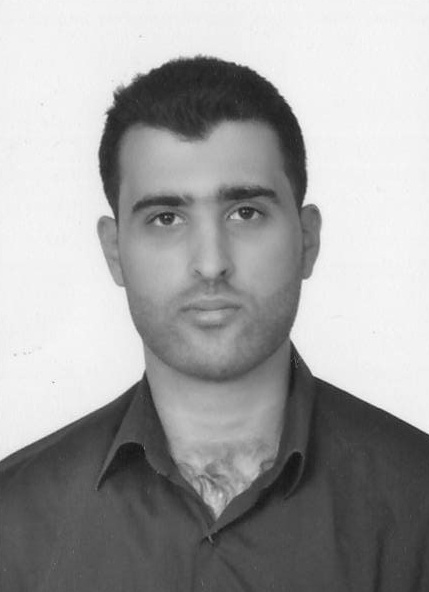
\includegraphics[scale=1]{mypicture.jpg}
\caption{Original picture (429X592)}
	\end{center}
\end{figure}
\begin{figure}[H]
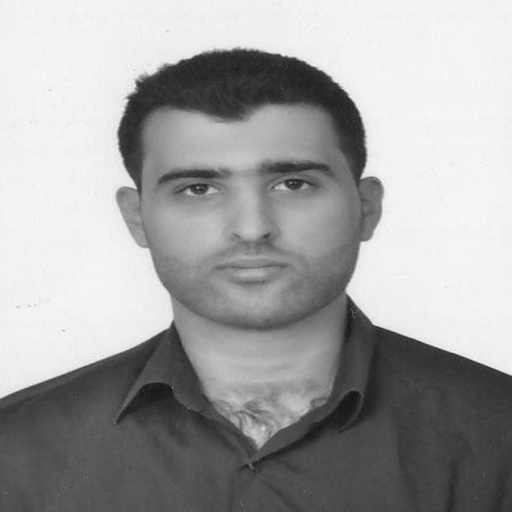
\includegraphics[scale=1]{mypicture_resized.jpg}
\caption{Image after resizing (512X512) using lanczos 4}
\end{figure}
\begin{figure}[H]
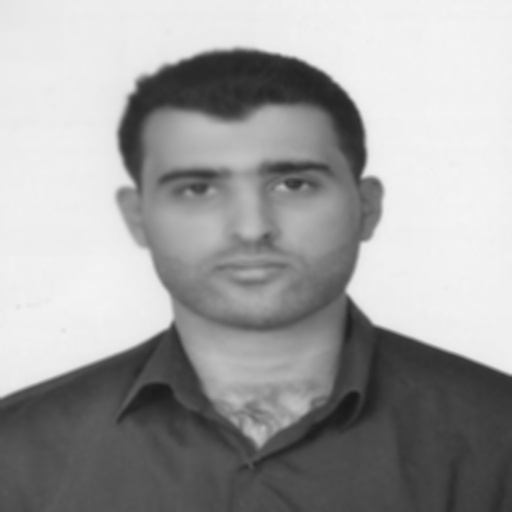
\includegraphics[scale=1]{blurred_piece_by_piece.jpg}
\caption{Image after blurring (512X512) patch size (16)}
\end{figure}
\textbf{Note: }The home work files,images,python code etc.. exist at \href{https://github.com/aqeel13932/IP/tree/master/hw4}{github}
\end{document}